\section{LTI-Systeme (S.29)}
\begin{list}{$\bullet$}{\setlength{\itemsep}{0cm} \setlength{\parsep}{0cm} \setlength{\topsep}{0cm}} 
	\item Lineare Systeme sind durch die Antworten auf die
	Basissignale bestimmt.
	\item Basissignale müssen linear unabhängig voneinander sein
	\item Alle Eingangs-Funktionen müssen durch eine Linearkombination der
	Basissignale darstellbar sein.\\ $\Rightarrow$ \textbf{Periode des Eingangssignals =	Anzahl Basissignale}
\end{list}
	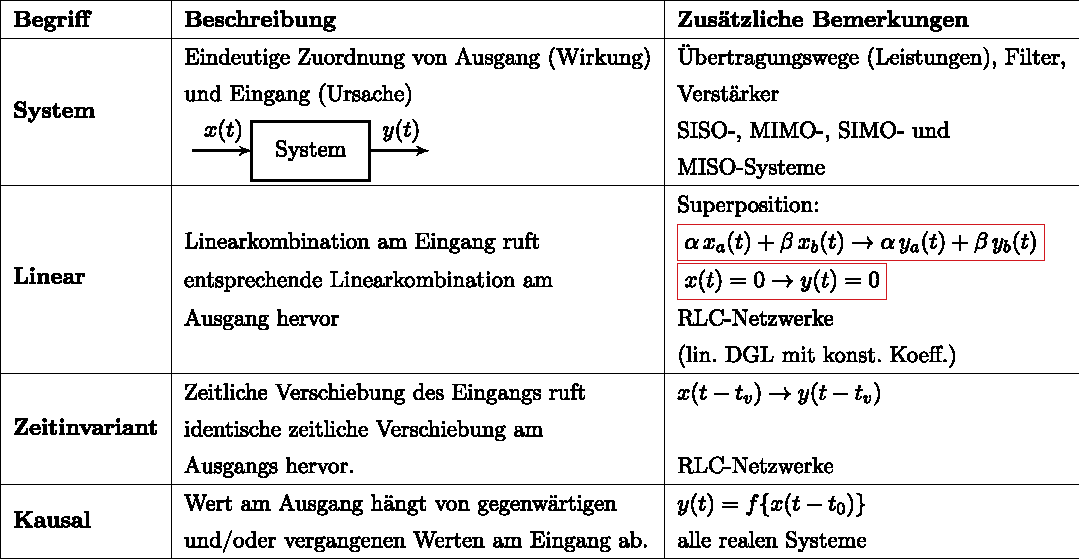
\includegraphics[width=0.9\textwidth]{content/05_LTI/tab_LTI.pdf}

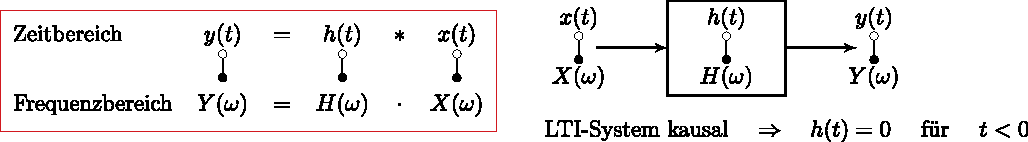
\includegraphics{content/05_LTI/Faltung_System.pdf}
\subsection{Verzerrungsfreies LTI-System S.33}
\vspace{.03cm}
Ein LTI System ist verzerrungsfrei wenn \efbox[linecolor=red]{$H(\omega) = k_a \cdot e^{-j\omega t_d}$} gilt. Der Amplitudengang muss konstant sein ($H(\omega) = k_a$) und der Phasengang eine lineare Funktion von $f$ bzw. $\omega$ sein. Für kausale Systeme muss \textbf{Verzögerung} $t_d > 0$ sein und damit fällt der Phasengang mit steigender Frequenz linear ab: $\varphi(\omega) = -t_d \cdot \omega$

\subsection{Dirac Impuls (Stösschen) S.30}
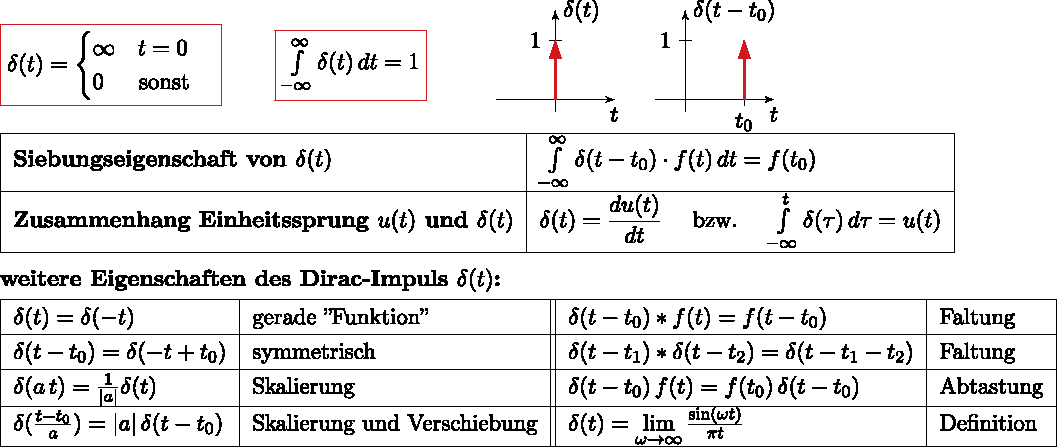
\includegraphics[width=.95\linewidth]{content/05_LTI/stoesschen.pdf}

\subsection{Signalmanipulationen}
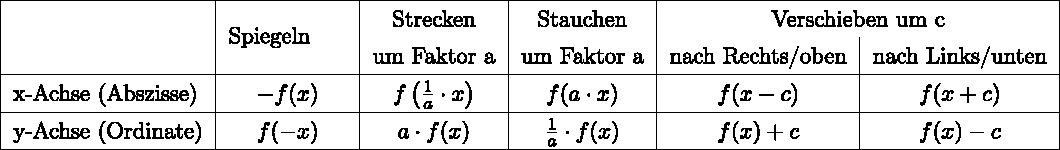
\includegraphics[width=\textwidth]{content/05_LTI/signalmanipulation.pdf}

\subsection{Grundlegende Funktionen S.30}
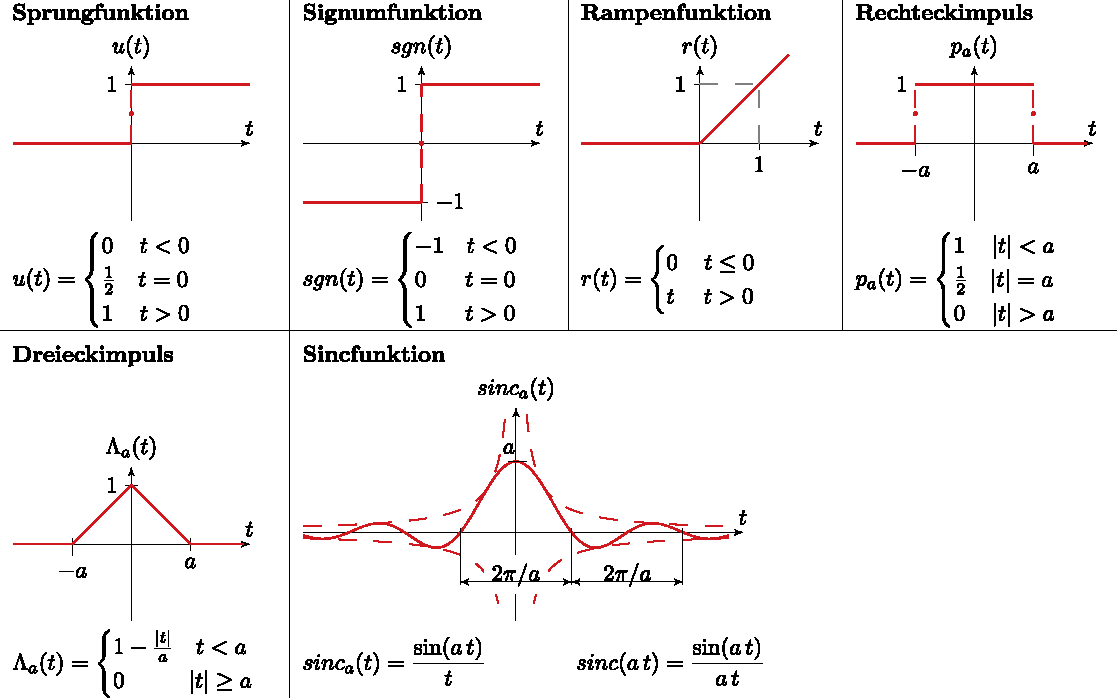
\includegraphics[width=\textwidth]{content/05_LTI/grundlegende_funktionen.pdf}

\subsection{Filtereigenschaften von LTI Systemen S.33}

\begin{minipage}{.4\linewidth}
	\begin{center}
		\begin{tabular}{|c|c|c|}
			\hline
			Tiefpass & Lowpass Filter & LPF \\
			\hline
			Hochpass & Highpass Filter & HPF \\
			\hline
			Bandpass & Bandpass Filter & BPF \\
			\hline
			Bandsperre & Bandstop Filter & BSF \\
			\hline
		\end{tabular}
	\end{center}
\end{minipage}
\begin{minipage}{.6\linewidth}
	Ideale Filter sind \textbf{akausal} und deshalb \textbf{nicht realisierbar}. Reale Filter stellen einen Kompromiss dar:
	\begin{list}{$\bullet$}{\setlength{\itemsep}{0cm} \setlength{\parsep}{0cm} \setlength{\topsep}{0cm}} 
		\item Filterflankensteilheit
		\item Dämpfung im Sperrbereich
		\item Flachem Frequenzgang im Durchlassbereich
		\item Linearität des Phasengangs
	\end{list}
\end{minipage}

\subsubsection{Bandbreite}
Die Bandbreite ist nur für \textbf{Tiefpass und Bandpassfilter} definiert. Bei realen Filtern wird üblicherweise die \textbf{\qty{3}{\dB} Eckfrequenz} angenommen, dabei erreicht die Amplitudendämpfung einen Wert von $k=\frac{1}{\sqrt{2}}$

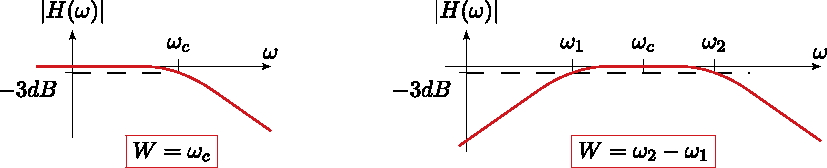
\includegraphics{content/05_LTI/tiefbandpassbandbreite.pdf}

\subsection{Quadraturfilter, Hilberttransformation S. 37}
Der Quadraturfilter ist ein Allpassfilter, dieser lässt die Amplitude unverändert und dreht nur die Phase um eine viertel Periode $-\frac{\pi}{2}$. Es resultiert eine grosse Verzögerung für tieffrequente Anteile und eine kleine für hochfrequente Anteile.

\vspace{.03cm}
\begin{minipage}{.5\linewidth}
\efbox[linecolor=red]{$H(\omega) = -j \cdot sgn(\omega) = \left\{
	\begin{matrix}
		e^{-j\pi /2} \;\; \omega > 0\\
		e^{+j\pi /2} \;\; \omega < 0
	\end{matrix}
	\right.$}
\end{minipage}
\begin{minipage}{.5\linewidth}
	\vspace{.03cm}
	\hspace{.01cm}
	\efbox[linecolor=red]{$h(t) = \frac{1}{\pi \cdot t}$}
\end{minipage}

